\section{Part a}
\begin{figure}[H]
	\centering
	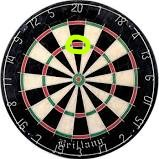
\includegraphics[scale=1.5]{Dartboard_colors.jpg}
	\caption{Dartboard with yellow circle around 60-point region}
\end{figure}

Assuming that all three darts could hit the dart board randomly, there is a finite (even though small) probability that all three will hit the triple score region (inner red-and-green ring) in the 20-point "slice" (see yellow circle in Fig.3.1). That would make each throw worth 60 points and therefore this would make a total possible score of 180 points for 3 throws. That would represent the highest possible score.\\
Now we design a Monte Carlo simulation for scoring three darts with the assumption of hitting the board at random and we list the scores of 5 sets of three-dart throws.
\[
\begin{bmatrix} 
      					Dart\#1 & Dart\#2 & Dart\#3 & Total \\
     					 16 & 8 & 25 & 49\\
					 1 & 14 & 0 & 15\\
					 25 & 0 & 15 & 40\\
					 0 & 11 & 0 & 11\\
					 0 & 9 & 12 & 21			  
\end{bmatrix}
\]

Thus, as we see, none of our random throws has given us the highest possible score. In fact, the highest score obtained in the simulation (49) is eleven points lower than the highest possible score that could be obtained by one throw in the triple region of the 20-point "slice."\\

\section{Part b}
Simulating the program 10,000 times give us the following mean value and standard deviation
$$
\mu = 34.1411
$$
$$
\sigma = 22.0310
$$
We can see that the mean value for 10,000 simulations is consistently different from what we would get by simply averaging the 5 sets of throws that we have obtained in Part a, in fact
$$
\frac{49+15+40+11+21}{5} = 27.2,
$$
which represents a value that is roughly 20\% smaller than the mean score obtained by simulating the program 10,000 times.

\section{Part c}

\begin{figure}[H]
	\centering
	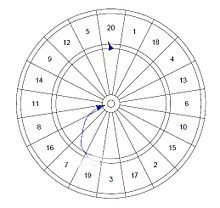
\includegraphics[scale=0.9]{Dartboard_optimal.jpg}
	\caption{Dartboard}
\end{figure}

Let's have a brief review of the most common rules followed in the game of darts.\\
The oche (line behind which the thrower must stand) should be 7 ft 9(1/2)in (2.37 m) from the face of the board.
Most games are usually played following the "501 up" rule. I.e. each player starts with 501 points and takes turns to throw 3 darts. The first player who reaches exactly 0 wins the game. It is a double out game, which means that players must hit a double that makes their score exactly zero to win the game. Moreover, if a player reduces the score to 1 or goes below to zero, the score is bust and his/her score is returned to that of his/her previous turn. If none of the players gets to zero in 20 turns, the player with the lower point wins.
If the scores are equal after 20 turns, the game will continue for another possible 10 turns.
During these extra turns, the player who gets to zero obviously wins. A player with lower score any time after the 20th turn also wins the match.
If the scores are equal after 20+10 turns, the match will end in a draw.\\
Thus, as we see, there are many variables that play into the game that have not been taken into account in our previous Monte Carlo simulation.\\
Assuming standard scoring, the optimal area to aim for on the dart board in order to maximise the player's score varies significantly based on the players' skill. The skilled player should aim for the centre of the T20 (the 20-point "slice") and as the player's skill decreases, their aim moves slightly up and to the left of the T20, according to $\textit{A Statistician Plays Darts}$, by R. Tibshirani, A. Price and J. Taylor.\\
So, we might want to modify our Monte Carlo Simulation by considering the players' different skill-sets and therefore their accuracy in their throws. For instance, we know from literature that for a player for perfect accuracy (practically extremely unlikely, but theoretically acceptable) the best place to aim is the center of the T20, whereas a player that throws randomly (amateur, first-time player) should aim into the centre of the dartboard, stopping a little lower and to the left of the bull's eye. So assuming that all players will try to maximise theirs scores in accordance to their different skills levels, we might want to run a simulation taking into account skill-sets, let's say having ability levels going from 1 to 10 (10 being the most-skilled), so that we could have a more realistic distribution of scores among players. For each throw, we might want to maximise the probability that each player will actually hit the section of the dartboard that he/she is aiming to, but we should also give a higher probability of that happening for better-skilled players and lower for not-so-skilled players.\\
So, for instance, let's assume that the most-skilled player (skill level 10) has a 96\% chance to hit the T20 for each throw. Then, the percentage of hitting the highest scoring region (the triple region) would be 20\% of the total chance for each throw, as there is less surface area to aim to, and same goes for the double region (as it has the same surface area of the triple region), and a 10\% chance to hit the bull's eye. Of the remaining 4\%, 99.9\% of chance to hit the regions next by and 0.1\% to not hit the dartboard or to hit the no-points region.\\
Let's give the least-skilled player (skill level 1) a 5\% probability to hit his desired target and a 50\% probability to hit the region of the dartboard that gives points (which means for every throw he has a 50\% chance to score zero points).\\
From these lower and upper limits we would build the conditions for all the remaining players (skill levels from 2 to 8). Then we would have to randomly extract, let's say, 5 players with different skill-sets and simulate a game among them.
Obviously there would be the necessity to take into account the fact that, as players either reach 1 point or go below zero, they bust and go back to the previous score. As best-skilled players would have a higher probability to win matches, they would also have a higher probability to find themselves in a critical situation with regard to their scores, which would require for them to change strategy in order to avoid busting.\\
These are some of the improvements that could be made to a have a more realistic simulation of a dartboard match.
%Now, to simplify our discussion, let's assume that the players are all professional or at least somewhat trained in the "sport" of darts, so that their skill-set is more or less uniform. So, all of them has trained himself/herself to get the most points from every single round, at least up until some arithmetic needs to be involved in order not to bust. So, most players will try to aim to the portion of the dartboard where they could get the most points, which is represented by the bull's eye (50 points worth of) straight up into the 20-point "slice", especially the triple and double region (which will be worth 60 and 40 points per throw respectively). Now, it is reasonable to assume that not all darts will end up in the desired spot, but, since the players are all well-trained, it is also reasonable to think that most of their darts will end up close to the desire spot. Let's say within 0.5 inches to their aim.%


